\chapter{Financial Instruments: Mortgages and Bonds}

\section{Mortgages}

\begin{definition}
    A \textbf{mortgage} is a loan secured by the collateral of real estate property. The borrower is obligated to pay back the loan in a specified period of time. If the borrower fails to make the payments, the lender can take possession of the property.
\end{definition}

\begin{definition}
    [Principle]
    The \textbf{principle} is the amount of money borrowed from the lender. In the case of a mortgage, the principle is the percent of the house's value that the borrower did not pay upfront.
\end{definition}

\begin{definition}
    [Down Payment]
    The \textbf{down payment} is the amount of money paid upfront by the borrower. The down payment is a percentage of the house's value.
\end{definition}

\begin{definition}
    [Loan to Value Ratio]
    The \textbf{loan to value ratio} is the ratio of the principle to the value of the house. The loan to value ratio is calculated as follows:
    \[
        \text{LTV} = \frac{\text{Principle}}{\text{House Value}}
    \]
\end{definition}

\begin{definition}
    [Amortization Period]
    The \textbf{amortization period} is the amount of time it takes to pay off the mortgage. The amortization period is typically 25 years.
\end{definition}

\begin{definition}
    [Mortgage Rate]
    The \textbf{mortgage rate} is the interest rate on the mortgage. The mortgage rate is typically 2-3\%.\\
    \textit{Note: The mortgage rate is given as an \textbf{annual rate}.}
\end{definition}

\begin{definition}
    [Mortgage Term]
    The \textbf{mortgage term} is the amount of time the mortgage rate is fixed. After which the mortgage rate is renegotiated.
    \\ The mortgage term is typically 5 years.
\end{definition}

\begin{example}
    [Mortgage Payment]
    Suppose you buy a house for \$500,000 with a 20\% down payment. You take out a mortgage with a 5\% interest rate, a 5 year term, and a 25 year amortization period. \\
    a) What is your monthly payment during this term?
    \begin{align*}
        P_1 &= 400,000 \quad &\text{(Principle)}\\
        i_1 &= 0.05 \quad &\text{(Mortgage Rate)}\\
        N_1 &= 25\times 12 = 300 \quad &\text{(Number of Payments)}\\
        A_1 &= P \cdot (A/P, i_1, N_2)\\
        &= \$ 2338
    \end{align*}    
    b) After the end of the term, the new mortgage rate is 6\%. What is your new monthly payment?
    \begin{align*}
        i_2 &= 0.06 \quad &\text{(New Mortgage Rate)}\\
        P_2 &= P_1\cdot (F/P, i_1, 5\times 12) &\text{(Principle after 5 years)}\\
        & - A_1\cdot (F/A, i_2, 5\times 12) &\text{(Payments after 5 years)}\\
        & = \$354,320 \\
        N_2 &= 20\times 12 = 240 \quad &\text{(Number of Payments)}\\
        A_2 &= P_2\cdot (A/P, i_2, N)\\
        &= \$ 2,538
    \end{align*}
\end{example}

\section{Bonds}

\begin{definition}
    [Bond]
    A \textbf{bond} is a fixed income instrument that represents a loan made by an investor to a borrower. The borrower is typically a corporation or government. The borrower agrees to pay the investor a fixed interest rate over a specified period of time (usually 10-30 years).
\end{definition}

\begin{definition}
    [Face Value]
    The \textbf{face value} is the amount of money the bondholder will receive at the end of the bond's term. The face value is also known as the \textbf{par value}.
\end{definition}

\begin{figure}[H]
    \centering
    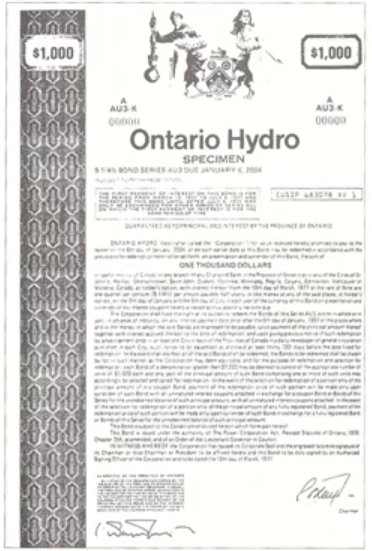
\includegraphics[width=0.5\textwidth]{LECTURE_3/bond-face.png}
    \caption{Bond Front/Face}
\end{figure}

\begin{definition}
    [Coupon Rate]
    The \textbf{coupon rate} is the interest rate that the bondholder will receive annually as a percentage of the face value. The coupon rate is typically 2-3\%.
\end{definition}

\begin{theorem}
    [Cash Flow Comparison]
    It is common that cash flows are compared to the current interest rate you would receive if you invested the same amount of money in a savings account. This is because the banks are considered to be the safest investment.
\end{theorem}

\subsection{Risk and Reward}
\begin{definition}
    [Yield Rate]
    The \textbf{yield rate} is the rate of return on an investment. The yield rate is the interest rate that makes the present value of the investment's cash flows equal to the bond's price. \\
    On the flip side, the yield rate is the amount you (or the market) is willing to pay for the investment due to it's perceived risk.
\end{definition}
\begin{example}
    [Bond Cash Flow Comparison]
    Suppose you buy a bond with a face value of \$1000, a coupon rate of 5\%, and a term of 10 years.\\
    The bank is paying 10\% interest. What is the equivalent amount you would need to put into the bank now in order to get the same cash flows?
    \begin{align*}
        i_{\text{Bank}} &= 0.1/2 = 0.05 \quad &\text{(Bank Rate Semi-annually)}\\
        i_{\text{Bond}} &= 0.05 \quad &\text{(Bond Rate)}\\
        N &= 10\times 2 = 20 \quad &\text{(Number of Payments)}\\
        A &= 1000\times i_{\text{Bond}} =\$ 46.25 &\text{(Semi-annual Payment)}\\
        F &= 1000 &\text{(Face Value)}\\
        P &= F\cdot (P/F, i_{\text{Bank}}, N) + A\cdot (P/A, i_{\text{Bank}}, N)\\
        & = \$ 953
    \end{align*}
    So, you would need to put \$953 in the bank to get the same cash flows as the bond. Do you trust the bond issuer as much as the bank? \\
    \textbf{Say that we don't trust the bond issuer as much as the bank.} \\
    Let's say the market is only willing to pay \$ 700 for the bond. What is the yield rate?
    \begin{align*}
        P &= 700 \quad &\text{(Bond Price)}\\
        i_{\text{yield}} &= ?\\
        P &= F\cdot (P/F, i_{\text{yield}}, N) + A\cdot (P/A, i_{\text{yield}}, N)\\
        i_{\text{yield}} &= 0.15\%
    \end{align*}
\end{example}

\section{Bonds Examples}


\begin{example}
    [Bond Price]
    A \$ 10,000 bond was bought that will mature in 8 years, it has a 12\% coupon payable quarterly. If the yield is 10\%, how much would you pay for the bond if it was for sale? \\
    \textbf{First we calculate the coupon payment:}
    \begin{align*}
        i &= 0.12/4 = 0.03 \quad &\text{(Coupon Rate)}\\
        A &= 10,000 \times 0.03 = \$ 300 &\text{(Quarterly Payment)}
    \end{align*}
    \textbf{Then we calculate the bond price:}
    \begin{align*}
        i_{\text{yield}} &= 0.1/4 = 0.025 \quad &\text{(Yield Rate)}\\
        N &= 8\times 4 = 32 \quad &\text{(Number of Payments)}\\
        P &= 300\cdot (P/A, 0.025, 32) + 10,000\cdot (P/F, 0.025, 32)\\
        &= \$ 11,092
    \end{align*}
\end{example}

